\documentclass[12pt,a4paper]{article}

\usepackage[T1]{fontenc}
\usepackage[margin=1in]{geometry}
\usepackage{amsmath,amssymb,amsthm,graphicx}
\usepackage{lmodern}
\usepackage{hyperref}
\usepackage{setspace}
\usepackage{fancyhdr}

\onehalfspacing

% Set up fancy header
\pagestyle{fancy}
\fancyhf{}
\fancyhead[L]{IYMC 2024 Qualification Round}
\fancyhead[R]{Solution E}
\fancyfoot{}
\renewcommand{\headrulewidth}{0.4pt}
\setlength{\headsep}{1cm}

\begin{document}

\title{\textbf{Solution: Problem E}}
\author{}
\date{}
\maketitle
\thispagestyle{fancy}

\noindent\textbf{Detailed solution for Problem E:}

We have two squares of equal side length \( a \).

- \(\mathbf{S_1}\): A square of side length \( a \), centered at the origin \((0,0)\) and aligned with the coordinate axes.

  This means:
  \[
  S_1: -\frac{a}{2} \le x \le \frac{a}{2} \quad\text{and}\quad -\frac{a}{2} \le y \le \frac{a}{2}.
  \]
  
  The vertices of \( S_1 \) are:
  \[
  A = \left(\frac{a}{2}, \frac{a}{2}\right), \quad B = \left(\frac{a}{2}, -\frac{a}{2}\right), \quad C = \left(-\frac{a}{2}, -\frac{a}{2}\right), \quad D = \left(-\frac{a}{2}, \frac{a}{2}\right).
  \]

  The area of \( S_1 \) is \( a^2 \).

\medskip

- \(\mathbf{S_2'}\) \textit{before rotation}:  
  We shall consider an axis-aligned square \( S_2' \) of side length \( a \), placed such that one of its vertices is at the origin \((0,0)\) and the square extends into the first quadrant. Without rotation, its vertices are:
  \[
  W'=(0,0), \quad X'=(a,0), \quad Y'=(a,a), \quad Z'=(0,a).
  \]

  This square \( S_2' \) also has area \( a^2 \). In this configuration, \( S_2' \) is not centered at the origin. Instead, it just has a vertex at the origin.

\medskip

\noindent\textbf{Now, Rotate \( S_2' \) by 45° Clockwise:}

We rotate the square \( S_2' \) by 45° \textbf{clockwise} about the origin as shown in the figure. A 45° clockwise rotation transforms a point \((x,y)\) as follows:

- Rotation by 45° clockwise can be represented by the transformation:
  \[
  (x',y') = \left(x\frac{\sqrt{2}}{2} + y\frac{\sqrt{2}}{2},\ -x\frac{\sqrt{2}}{2} + y\frac{\sqrt{2}}{2}\right).
  \]

\medskip

% Insert the Desmos figure here
\begin{figure}[h!]
\centering
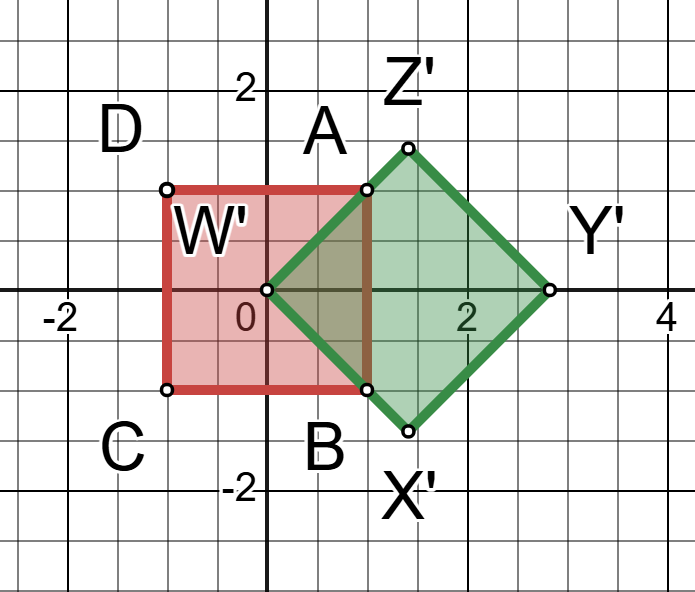
\includegraphics[width=0.55\textwidth]{desmos_figure.png} % <-- replace with your actual image file name
\caption{Desmos plot of $S_1$ (red) and $S_2$ (green) after rotating $S_2'$ by 45° clockwise about the origin.}
\label{fig:desmos}
\end{figure}

\medskip

We now apply this rotation to each vertex of \( S_2' \):

1. \(W'=(0,0)\):
   \[
   W = \left(0\cdot\frac{\sqrt{2}}{2} + 0,\ -0\cdot\frac{\sqrt{2}}{2}+0\right) = (0,0).
   \]

2. \(X'=(a,0)\):
   \[
   X = \left(a\frac{\sqrt{2}}{2} + 0,\ -a\frac{\sqrt{2}}{2}+0\right) = \left(\frac{a}{\sqrt{2}}, -\frac{a}{\sqrt{2}}\right).
   \]

3. \(Y'=(a,a)\):
   \[
   Y = \left(a\frac{\sqrt{2}}{2} + a\frac{\sqrt{2}}{2},\ -a\frac{\sqrt{2}}{2} + a\frac{\sqrt{2}}{2}\right).
   \]

   We shall combine terms inside each coordinate:
   - For \(x'\): \(a\frac{\sqrt{2}}{2} + a\frac{\sqrt{2}}{2} = a\sqrt{2}\).
   - For \(y'\): \(-a\frac{\sqrt{2}}{2} + a\frac{\sqrt{2}}{2} = 0\).

   Thus:
   \[
   Y = (a\sqrt{2}, 0).
   \]

4. \(Z'=(0,a)\):
   \[
   Z = \left(0 + a\frac{\sqrt{2}}{2},\ -0 + a\frac{\sqrt{2}}{2}\right) = \left(\frac{a}{\sqrt{2}}, \frac{a}{\sqrt{2}}\right).
   \]

After rotation, the square \( S_2 \) (rotated version of \( S_2' \)) has vertices:
\[
W=(0,0), \quad X=\left(\frac{a}{\sqrt{2}}, -\frac{a}{\sqrt{2}}\right), \quad Y=(a\sqrt{2},0), \quad Z=\left(\frac{a}{\sqrt{2}}, \frac{a}{\sqrt{2}}\right).
\]

The area of \( S_2 \) remains \( a^2 \).

Note: \( S_2 \) is no longer axis-aligned nor centered at the origin. It has one vertex at the origin and is tilted 45° clockwise.

\medskip

\noindent\textbf{Visualizing the Overlap:}

- \( S_1 \) is a square centered at the origin, with corners at \((\pm a/2,\pm a/2)\).
- \( S_2 \), after the 45° clockwise rotation, has a vertex at \(W=(0,0)\), stretches to the right (positive \(x\)-direction) up to \(Y=(a\sqrt{2},0)\), and also has vertices \(Z\) in the first quadrant and \(X\) in the fourth quadrant.

This configuration implies:
- \( S_2 \) extends into both the first quadrant (Q1) and fourth quadrant (Q4), with the origin as a pivot point.
- We will analyze the intersection \( S_1 \cap S_2 \) quadrant by quadrant.

\medskip

\noindent\textbf{Defining the Edges of \( S_2 \):}

The rotated square \( S_2 \) has vertices in the order \( W \to Z \to Y \to X \to W \).

1. Edge \(WZ\): Connects \(W=(0,0)\) to \(Z=(a/\sqrt{2}, a/\sqrt{2})\).
   - Slope = \(\frac{a/\sqrt{2}-0}{a/\sqrt{2}-0}=1\).
   Equation: \(y=x\).

2. Edge \(ZY\): Connects \(Z=(a/\sqrt{2}, a/\sqrt{2})\) to \(Y=(a\sqrt{2},0)\).
   Find the slope:
   \[
   \text{slope} = \frac{0 - a/\sqrt{2}}{a\sqrt{2} - a/\sqrt{2}}
   = \frac{-a/\sqrt{2}}{a(\sqrt{2}-1/\sqrt{2})}.
   \]
   Simplify denominator:
   \(\sqrt{2}-\frac{1}{\sqrt{2}} = \frac{2-1}{\sqrt{2}}=\frac{1}{\sqrt{2}}\).

   Thus denominator = \(a/\sqrt{2}\).

   Slope = \(\frac{-a/\sqrt{2}}{a/\sqrt{2}} = -1\).

   Line through \(Z\):
   \[
   y - \frac{a}{\sqrt{2}} = -1\Bigl(x - \frac{a}{\sqrt{2}}\Bigr) \implies y = -x + a\sqrt{2}.
   \]

3. Edge \(YX\): Connects \(Y=(a\sqrt{2},0)\) to \(X=(a/\sqrt{2}, -a/\sqrt{2})\).
   Slope:
   \[
   \frac{-a/\sqrt{2}-0}{a/\sqrt{2}-a\sqrt{2}}
   = \frac{-a/\sqrt2}{\,a/\sqrt2 - a\sqrt{2}\,}.
   \]
   Factor out \(a/\sqrt{2}\):
   \[
   a/\sqrt{2}-a\sqrt{2} = a\Bigl(\frac{1}{\sqrt{2}}-\sqrt{2}\Bigr) = a\Bigl(\frac{1-2}{\sqrt{2}}\Bigr) = \frac{-a}{\sqrt{2}}.
   \]
   Numerator = \(-a/\sqrt{2}\), Denominator = \(-a/\sqrt{2}\). Slope = 1.

   Equation through \(Y\):
   \[
   y = x - a\sqrt{2}.
   \]

4. Edge \(XW\): Connects \(X=(a/\sqrt{2}, -a/\sqrt{2})\) to \(W=(0,0)\).
   Slope:
   \[
   \frac{0 + a/\sqrt{2}}{0 - a/\sqrt{2}} = \frac{a/\sqrt{2}}{-a/\sqrt{2}} = -1.
   \]
   Equation through \(W\):
   \[
   y = -x.
   \]

So the edges are:
\[
WZ: y=x, \quad ZY: y=-x+a\sqrt{2}, \quad YX: y=x - a\sqrt{2}, \quad XW: y=-x.
\]

\medskip

\noindent\textbf{Intersection with \( S_1 \):}

Recall \( S_1 \):
\[
- \frac{a}{2}\le x \le \frac{a}{2}, \quad -\frac{a}{2}\le y \le \frac{a}{2}.
\]

\( S_2 \) occupies a region around the origin but rotated. Let’s consider each relevant quadrant.

\medskip

\noindent\textbf{Intersection in the First Quadrant (Q1):}

In Q1:
- \( S_1 \) constraints: \(0 \le x \le a/2,\ 0 \le y \le a/2.\)
- In Q1, \( S_2 \) near the origin is bounded below by \(WZ: y=x\). To be inside \( S_2 \), we must have \( y \ge x \) in this region.

The upper edges of \( S_2 \) in Q1 are very high (like \( y=-x+a\sqrt{2}\)), which is well above \( y=a/2 \) since \( a\sqrt{2} > a/2 \). Thus, the top boundary in Q1 intersection is actually the top of \( S_1 \), i.e.\ \( y=a/2 \).

Hence, in Q1, the intersection region is:
\[
\{(x,y): 0\le x\le a/2,\ x \le y \le a/2\}.
\]

This is a right triangle with vertices:
\((0,0), (0,a/2), (a/2,a/2)\).

Area in Q1:
\[
\frac{1}{2}\times\frac{a}{2}\times\frac{a}{2}=\frac{a^2}{8}.
\]

\medskip

\noindent\textbf{Intersection in the Second Quadrant (Q2):}

We check if \( S_2 \) extends into Q2 with \( y>0 \). From the vertex configuration and the shape after rotation, \( S_2 \) mainly extends into Q1 and Q4. It does not have any part that goes into Q2 above the x-axis. Thus, there is no intersection region in Q2.

\medskip

\noindent\textbf{Intersection in the Fourth Quadrant (Q4):}

In Q4:
- \( S_1 \) constraints: \(0 \le x \le a/2,\ -a/2 \le y \le 0.\)
- In Q4, the relevant edge of \( S_2 \) near the origin is \(XW: y=-x\). To be inside \( S_2 \) in Q4, we must have \( y \ge -x \) because the polygon opens above the line \( y=-x \) in that region.

We know \( y \le 0 \) from \( S_1 \), and \(-a/2 \le y \le 0\).

At \( x=0 \), \( y \ge 0 \) and \( y\le 0 \) implies \( y=0 \).

At \( x=a/2 \), since \( y\ge -x \) implies \( y\ge -a/2 \), and from \( S_1 \), \( y \le 0 \). This forms another right triangle with vertices:
\((0,0), (0,-a/2), (a/2,-a/2)\).

Area in Q4:
\[
\frac{1}{2}\times\frac{a}{2}\times\frac{a}{2} = \frac{a^2}{8}.
\]

\medskip

\noindent\textbf{No Intersection in the Third Quadrant (Q3):}

Since \( S_2 \) does not extend below \( y=0 \) in a manner that would intersect \( S_1 \) in Q3, there is no intersection there.

\medskip

\noindent\textbf{Total Intersection Area:}

We have:
- Q1 intersection area: \( a^2/8 \)
- Q4 intersection area: \( a^2/8 \)
- Q2: No intersection
- Q3: No intersection

Total intersection:
\[
A(S_1 \cap S_2) = \frac{a^2}{8} + \frac{a^2}{8} = \frac{a^2}{4}.
\]

\medskip

\noindent\textbf{Non-Overlapping Area of \( S_2 \):}

The area of \( S_2 \) is \( a^2 \). The intersection is \( a^2/4 \). Thus:
\[
A_{\text{non-overlap}} = A(S_2) - A(S_1 \cap S_2) = a^2 - \frac{a^2}{4} = \frac{3a^2}{4}.
\]

\medskip

\noindent\textbf{Final Answer:}
\[
\boxed{\mathbf{A(S_1 \cap S_2) = \frac{a^2}{4}\ \text{and}\ A_{\text{non-overlap}} = \frac{3a^2}{4}}}
\]

\bigskip

\noindent\textbf{Mathematical Concepts Involved in Problem E...}
\begin{itemize}
\item \textbf{Coordinate Plane Visualization:} Plotting squares $S_1$ and $S_2$ to see their relative positions.
\item \textbf{Square Geometry:} Familiarity with side length, diagonals, and areas of squares.
\item \textbf{Rotation Transformations:} A $45^\circ$ clockwise rotation formula in coordinates.
\item \textbf{Line Equations and Slopes:} Identifying the boundaries of $S_2$ after rotation by computing slopes and line equations.
\item \textbf{Intersection/Overlap Computation:} Splitting the intersection region by quadrants and summing triangular areas.
\item \textbf{Area Computations:} Using right triangles for partial overlaps and subtracting from the total area.
\item \textbf{Final Subtraction for Non-overlap:} $a^2 - \frac{a^2}{4} = \frac{3a^2}{4}$.
\end{itemize}

\bigskip
\noindent\hrulefill
\begin{center}
\textbf{************* END OF SOLUTION: E *************}
\end{center}
\hrulefill

\end{document}
